\documentclass[12pt]{article}

\usepackage{sbc-template}

\usepackage{setspace}
\usepackage{graphicx}


\usepackage{amsmath,amsfonts,amsthm,amssymb}         % fontes matemáticas, teoremas e etc.
\usepackage{latexsym}                                % mais símbolos matemáticos
\usepackage{cancel}
%\usepackage[portugues,algoruled,lined]{algorithm2e}  % excelente ambiente p/ escrever algoritmos
\usepackage{tabularx}                                % tabelas com diversas formas
\usepackage{multicol}                                % tabelas com multiplas colunas
\usepackage{multirow}                                % tabelas com multiplas linhas
\usepackage{booktabs}                                % tabelas profissionais
\usepackage{longtable}                               % tabelas longas
\usepackage{dcolumn}                                 % tipos especiais de colunas
\usepackage{lscape}                                  % página no formato paisagem
\usepackage{graphicx}                                % diversas configurações de imagens
\usepackage[normalem]{ulem}
\usepackage{fancyhdr}

\usepackage{geometry}
\usepackage{chngpage}


\usepackage[brazil]{babel}   
\usepackage[utf8]{inputenc}
\usepackage{algorithm2e}
     
\sloppy

\title{titulo aqui}

\author{Sérgio Luis O. B. Correia, Vinícius Moura Romão}


\address{Mestrado Acadêmico em Ciência da Computação (MACC)\\
  Universidade Estadual do Ceará (UECE).
\email{\{sergio, vinicius.romao\}@larces.uece.br} 
}

\begin{document} 

\maketitle

     
\begin{resumo} 
\end{resumo}


% formigas e otimizacao (aco)
\section{A otimização combinatória e as colônias de formigas}
\label{chapter:aco}

\subsection{Introdução}

No início da década de 1990, a otimização combinatória com colônias de formigas
(ACO, \textit{Ant Colony
Optimization}) \cite{dorigo1992optimization, dorigo1991positive, dorigo1996ant} surgiu como uma
nova técnica bioinspirada voltada para a solução de problemas difíceis
de otimização combinatória. ACO é uma metaheurística \cite{glover2003handbook},
ou seja, um algoritmo aproximado usado para obter soluções suficientemente
boas para problemas difíceis de otimização combinatória em tempo computacional
razoável. A fonte de inspiração para a metaheurística ACO foi o comportamento
forrageiro das formigas reais. Quando estão procurando por comida, as formigas
inicialmente exploram a área próxima ao seu formigueiro de forma aleatória.
Assim que uma formiga descobre alguma fonte de comida, ela avalia a fonte e
transporta um pouco de volta para o formigueiro. Nesse caminho de volta, a
formiga deposita uma trilha de feromônios --
substâncias químicas capazes de despertar reações fisiológicas ou
comportamentais em outros membros de uma mesma espécie que estejam num
determinado raio de espaço físico ocupado pelo excretor
\cite{karlson1959pheromones}. A quantidade de feromônio depositada, que pode
depender da quantidade e qualidade da comida, vai guiar outras formigas até a
fonte de comida. A comunicação indireta entre as formigas por meio das trilhas
de feromônios as torna capazes de encontrar o caminho mais curto entre o
formigueiro e a fonte de comida \cite{deneubourg1990self}. Essa característica
das colônias de formigas reais é explorada em colônias de formigas
artificiais, sendo a base da ACO. A Figura \ref{fig:formigueiro} mostra essa
característica. Em (i), vê-se uma formiga retornando da fonte de comida para o
formigueiro, deixando um rastro de feromônio pelo caminho percorrido. Em (ii)
são retratadas várias formigas indo do formigueiro à fonte de comida por
caminhos diferentes, e marcando esses caminhos com feromônio. As formigas que
escolhem o menor caminho retornam primeiro, e o nível de feromônio nesta
trilha vai se tornando mais acentuado com o tempo, aumentando a probabilidade
de futuras formigas escolherem esse caminho. (iii) mostra essa convergência,
onde, após algum tempo, a maior parte das formigas passa a utilizar o caminho
mais curto.

\begin{figure}
\centering
 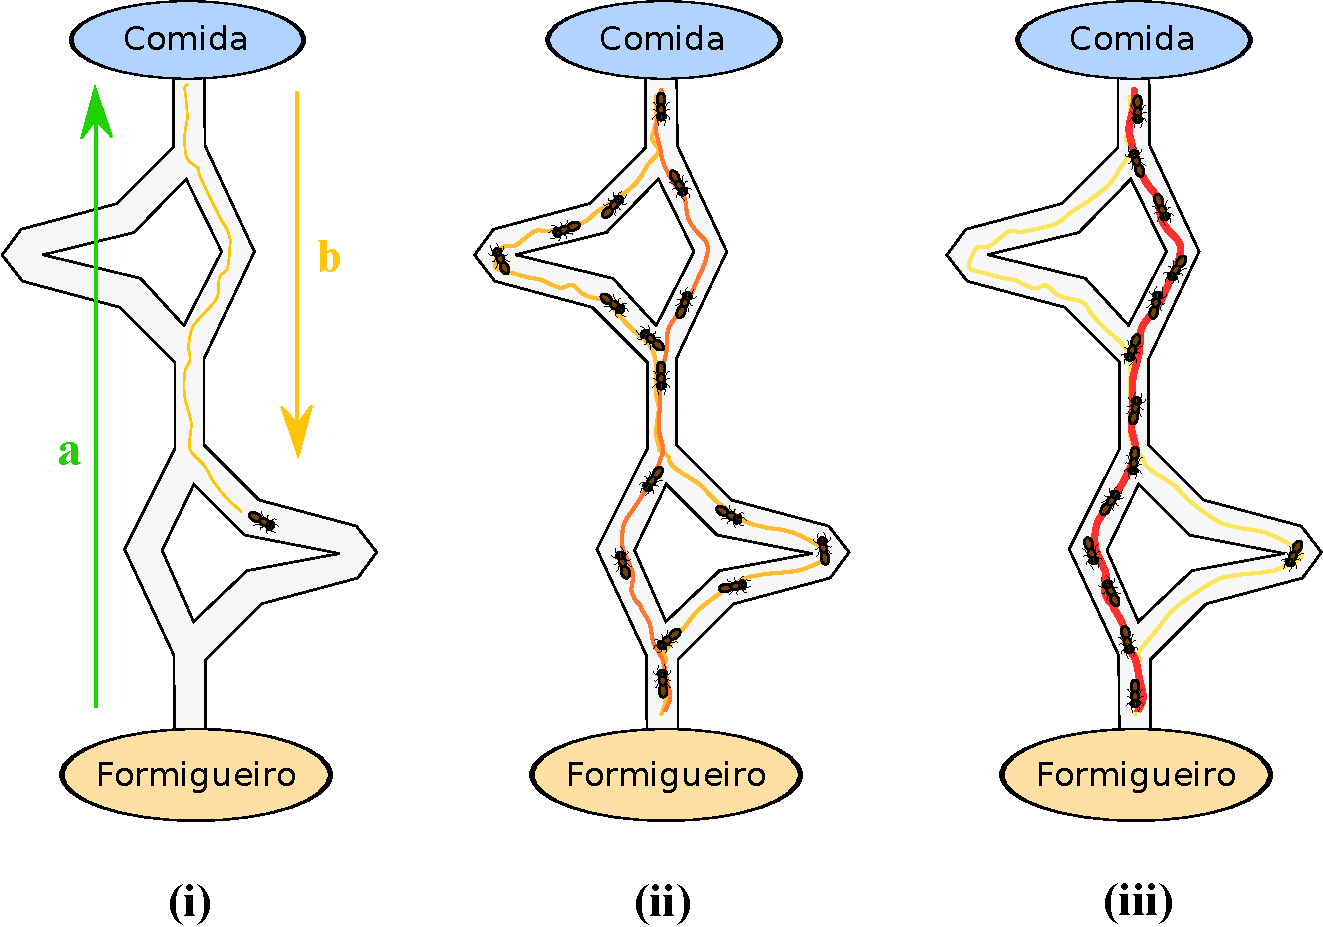
\includegraphics[scale=0.5]{fig/formigueiro-crop.pdf}
\caption{Colônia de formigas}
\label{fig:formigueiro}
\end{figure}


\subsection{Otimização combinatória}
A otimização combinatória é um ramo da matemática aplicada e da ciência da
computação que lida com a solução de problemas que podem ser catacterizados
como possuindo uma estrutura discreta ou combinatória. Estes problemas são
modelados com uma função objetivo e envolvem achar valores para variáveis
discretas tal que seja encontrada uma solução ótima para essa função objetivo.
Muitos dos problemas de otimização de importância teórica e prática são de
natureza combinatória, como por exemplo encontrar o melhor esquema de roteamento
de pacotes em uma rede, a melhor maneira de se alocar professores e disciplinas ou a
melhor maneira de se visitar um determinado conjunto de lugares diferentes. 

Um problema de otimizaçao combinatória ou é de maximização ou de minimização, e
tem associado um conjunto de instâncias do problema. Aqui, \textit{problema} se
refere à pergunta a ser respondida, geralmente contendo vários parâmetros ou
variáveis com valores não especificados. Uma \textit{instância} se refere a um
problema com os valores especificados para cada parâmetro.

Formalmente, um problema de otimização combinatória $\Pi$ é uma tripla
$(\mathcal{S}, f, \Omega)$, onde $\mathcal{S}$ é o conjunto de soluções, $f$ é
a função objetivo que atribui um valor $f(s)$ a cada solução $s \in
\mathcal{S}$, e $\Omega$ é um conjunto de restrições. As soluções pertencentes
ao conjunto $\tilde{\mathcal{S}} \subseteq \mathcal{S}$ que satisfazem às
restrições $\Omega$ são chamadas soluções viáveis. A idéia é encontrar uma
solução $s^{*}$, viável, que seja um ótimo global, ou seja, ótima dentre
todas as soluções viáveis. Num problema de maximização, $s^{*}$ seria a solução
viável com o maior valor da função objetivo $f$, ao passo que, num problema de
minimização, $s^{*}$ seria a solução viável com o menor valor de $f$.

\subsection{O que é uma metaheurística?}
Uma metaheurística é um conjunto de conceitos algorítmicos que podem ser usados
para definir métodos heurísticos aplicáveis a uma diversidade de problemas
\cite{975277}. Uma metaheurística seria então um \textit{framework} algorítmico
que pode ser aplicado a diferentes problemas de otimização com relativamente
poucas modificações para torná-lo adaptado ao problema específico.

Como exemplos de metaheurísticas podemos citar algoritmos evolucionários, como
o \textit{Non-dominated Sorting Genetic Algorithm} (NSGA)
\cite{Srinivas94multiobjectiveoptimization}, o NSGA-II \cite{deb2002fast}, o
\textit{Strength Pareto Evolutionary Algorithm} (SPEA)
\cite{zitzler1998evolutionary} e o SPEA-II \cite{zitzler2001spea2}; algoritmos
probabilísticos, como o \textit{Bayesian Optimization Algorithm} (BOA)
\cite{Cantu-Paz98linkageproblem}, o \textit{Expectation-maximization
algorithm} (EM) \cite{moon1996expectation} e o \textit{Compact Genetic
Algorithm} \cite{harik1998compact}; algoritmos estocásticos, como o
\textit{Tabu Search} \cite{glover1990tabu}; e também algoritmos baseados em
inteligência coletiva, como algoritmos baseados em abelhas
\cite{teodorovic2005bee}, cupins \cite{roth2003termite}, e finalmente, em
formigas, \textit{Ant Colony Optimization} (ACO) \cite{dorigo1992optimization},
que será detalhado na próxima seção.

\subsection{Otimização combinatória com colônias de formigas - a metaheurística}
\label{sec:atsp}
Algoritmos ACO são procedimentos de busca
estocástica centrados em um modelo de feromônio, que é usado para tomar
amostras -- probabilisticamente -- dentro de um espaço de busca.

Como exemplo, vamos formular o problema do caixeiro viajante assimétrico
(ATSP,
\textit{Assymetric Traveling Salesman Problem}) a seguir. O problema em si
consiste em um grafo dirigido, completamente conectado $G(V, A)$, com um peso
positivo $d_{ij}$ associado a cada arco $a_{ij} \in A$. Os nós do grafo
representam cidades, e os pesos dos arcos, as distâncias entre elas. O objetivo
é encontrar, dentre todos os ciclos Hamiltonianos \footnote{Um ciclo ou caminho
hamiltoniano é um caminho que permite passar por todos os vértices de um grafo
G não repetindo nenhum, ou seja, passar por cada nó uma e apenas uma vez.} de
$G$, o de custo mínimo, o custo sendo a soma dos pesos de todos os seus arcos.
Este problema de otimização combinatória pode ser modelado da seguinte forma:
cada cidade $i \in V$ é modelada por uma variável de decisão $X_{i}$ cujo
domínio consiste de um valor $v_{i}^{j}$ para cada arco $a_{ij}$. A instância
de uma variável $X_{i} = v_{i}^{j}$ significa que o arco $a_{ij}$ é parte da
solução considerada. O conjunto de restrições é definido tal que somente
soluções candidatas que correspondam aos ciclos Hamiltonianos de $G$ são
soluções válidas. O conjunto de componentes de soluções $\mathcal{C}$ consiste
de um componente de solução $c_{i}^{j}$ para cada combinação de variável
$X_{i}$ e valor de domínio $v_{i}^{j}$, e o modelo de feromônio $\mathcal{T}$
consiste de uma trilha de feromônio $\mathcal{T}_{i}^{j}$, com um valor
$\tau_{i}^{j}$ associado a cada componente de solução $c_{i}^{j}$. 

\subsubsection{Um framework ACO simples}
O algoritmo \ref{algo:aco} mostra o \textit{framework} de um algoritmo ACO
básico, que funciona como segue: A cada iteração, $n_{a}$ formigas
probabilisticamente constróem soluções para o problema de otimização
combinatória considerado, explorando um dado modelo de feromônio, e
, opcionalmente, um procedimento de busca local é aplicado às soluções
construídas. Finalmente, antes da próxima iteração, algumas das soluções são
utilizadas na execução da atualização de feromônio. Este \textit{framework},
que foi descrito em \cite{dorigo2005ant}, será explicado com mais detalhes a
seguir.

\begin{algorithm}[h]
\label{algo:aco}
\caption{\textit{Framework} de um algoritmo ACO básico}
\Entrada{Uma instância $\mathcal{P}$ de um problema de otimização combinatória}
Inicializa os Feromônios($\mathcal{T}$)\;
$s_{melhor} \gets NULL$\;
\Enqto{condições de saída não forem satisfeitas}{
$\mathcal{C}_{iter} \gets \emptyset$\;
\Para{$i = 1, \ldots, n_{a}$} {
$s \gets$ Constrói Solução($\mathcal{T}$)\;
\Se{$s$ é uma solução válida} {
$s \gets$ Busca Local($s$) /* opcional */\;
\Se{($f(s) < f(s_{melhor})$) ou ($s_{melhor} = NULL$)} {
$s_{melhor} \gets s$\;
}
$\mathcal{C}_{iter} \gets \mathcal{C}_{iter} \cup \{s\}$
}
}
Atualiza Feromônio($\mathcal{T}, \mathcal{C}_{iter}, s_{melhor}$)\;
}
\Saida{A melhor solução até o momento, $s_{melhor}$}
\end{algorithm}

Inicializa os Feromônios($\mathcal{T}$). No início do algoritmo, os valores de
feromônio são todos inicializados com uma constante $c > 0$. 

Constrói Solução($\mathcal{T}$). O componente fundamental de qualquer algoritmo
ACO é uma heurística construtiva para a contrução probabilística das soluções.
Uma heurística construtiva monta soluções como sequências de elementos do
conjunto finito de componentes de solução $\mathcal{C}$. A construção de uma
solução começa com um conjunto vazio de soluções parciais $s_{parcial} =
\langle \rangle$, e a cada passo da construção, o conjunto de soluções parciais
é estendido adicionando-se um componente de solução viável do conjunto
$\mathcal{R}(s_{parcial}) \subseteq \mathcal{C} \setminus \{s_{parcial}\}$.
Este conjunto é determinado a cada passo do mecanismo de construção da solução
de modo que as restrições do problema são satisfeitas. O processo de construção
de soluções pode ser visualizado como o caminhamento no chamado grafo de
construção $G_{c} = (\mathcal{C}, \mathcal{L})$, que é um grafo completamente
conectado, cujos vértices são os componentes de solução em $\mathcal{C}$ e
cujas arestas são os elementos de $\mathcal{L}$. Os caminhamentos permitidos em
$G_{c}$ são definidos implicitamente pelo mecanismo de construção de solução
que define o conjunto $\mathcal{R}(s_{parcial})$ com respeito à solução parcial
$s_{parcial}$. A escolha de um componente de solução $c_{i}^{j} \in
\mathcal{R}(s_{parcial})$ é, em cada passo de construção, feito
probabilisticamente com respeito ao modelo de feromônio adotado. A
probabilidade para a escolha $c_{i}^{j}$ é proporcional a
$[\tau_{i}^{j}]^{\alpha} \cdot [n(c_{i}^{j})]^{\beta}$, onde $n$ é uma função
que atribui a cada componente de solução válida um valor heurístico que é
também conhecido como \textit{informação heurística}. Os valores dos parâmetros
$\alpha$ e $\beta$, $\alpha > 0$ e $\beta > 0$, determinam a importância
relativa dos valores de feromônio e da informação heurística. A informação
heurística é opcional, mas geralmente necessária quando se pretende alcançar
uma alta performance do algoritmo. Na maioria dos algoritmos ACO, as
probabilidades de se escolher o próximo componente de solução -- também chamada
de probabilidade de transição -- são definidas como segue:
\begin{equation}
\label{eq:acoprob}
P(c_{i}^{j} \mid s_{parcial}) = \frac{[\tau_{i}^{j}]^{\alpha} \cdot
[n(c_{i}^{j})]^{\beta}}{\sum_{c_{k}^{l} \in \mathcal{R}(s_{parcial})}
[\tau_{i}^{j}]^{\alpha} \cdot [n(c_{i}^{j})]^{\beta}}, \forall c_{i}^{j} \in
\mathcal{R}(s_{parcial})
\end{equation}

Na prática, há diversas formas de se escolher as probabilidades de transição,
mas a ilustrada em (\ref{eq:acoprob}) é tida como tradicional por ter sido
utilizada nos primeiros algoritmos ACO propostos, \cite{dorigo1991positive} e
\cite{dorigo1996ant}.

Voltando ao ATSP, definido em \ref{sec:atsp}, vamos denotar por $\mathcal{I}$ o
conjunto de índices da variável de decisão atual e das variáveis de decisão que
já têm um valor atribuído. A construção da solução começa com um conjunto de
soluções parciais vazio, $s_{parcial} = \langle \rangle$, com $i_{c} \in \{1,
\ldots, |V|\}$ escolhido aleatoriamente com $\mathcal{I} = \{i_{c}\}$. O índice
da primeira variável de decisão é armazenado na variável $i_{primeira}$. Então,
em cada dos $|V|-1$ passos de construção, um componente de solução $c_{i}^{j}
\in \mathcal{R}(s_{parcial})$ é adicionado à solução parcial, onde
$\mathcal{R}(s_{parcial}) = \{c_{i_{c}}^{k}\}\ |\ k \in \{1, \ldots, |V|\}
\setminus \mathcal{I}\}$. Isto significa que em cada passo de construção, um
valor de domínio é escolhido para a variável de decisão com índice $i_{c}$. Uma
vez que o componente de solução $c_{i_{c}}^{j}$ seja adicionado a
$s_{parcial}$, $i_{c}$ recebe o valor $j$. As probabilidades de transição
usadas em cada um dos primeiros $|V|-1$ passos de construção são as definidas
pela equação (\ref{eq:acoprob}). No ATSP, a informação heurística pode ser
definida como $n(c_{i}^{j}) = d_{ij}^{-1}$ (esta escolha dá preferência aos
menores caminhos). O último passo de construção consiste em adicionar o
componente de solução $c_{i_{c}}^{i_{primeira}}$ à solução parcial
$s_{parcial}$, que corresponde ao fechamento do ciclo Hamiltoniano.

Busca Local($s$). Um procedimento de busca local pode ser aplicado para
melhorar as soluções construídas pelas formigas. O uso de tal procedimento é
opcional, mas experimentos mostraram que, quando disponível, seu uso melhora o
desempenho geral do algoritmo \cite{dorigo2005ant}.

Atualiza Feromônio($\mathcal{T}, \mathcal{C}_{iter}, s_{melhor}$). A idéia por
trás da regra de atualização de feromônio é aumentar o nível de feromônio das
melhores soluções. Segundo \cite{dorigo2005ant}, a maioria dos algoritmos ACO
utiliza uma variação da regra de atualização (\ref{eq:acoupdate}).
\begin{equation}
\label{eq:acoupdate}
\tau_{i}^{j} \gets (1 - \rho) \cdot \tau_{i}^{j} +
\frac{\rho}{\mathcal{C}_{atualizacao}} \cdot \sum_{\{s \in
\mathcal{C}_{atualizacao} | c_{i}^{j} \in s\}} F(s),
\end{equation}

para $i = 1, \ldots n$, e $j = 1, \ldots |D_{i}|$. Instâncias desta regra de
atualização são obtidas com diferentes especificações de
$\mathcal{C}_{atualizacao}$, que é um subconjunto de $\mathcal{C}_{iter} \cup
\{s_{melhor}\}$, onde $\mathcal{C}_{iter}$ é o conjunto de soluções que foram
construídas na iteração atual, e $s_{melhor}$, a melhor solução até o momento.
O parâmetro $\rho \in (0, 1]$ é conhecido como \textit{taxa de evaporação}, e
tem a função de decrementar todos os valores de feromônio de modo uniforme. De
um ponto de vista prático, a evaporação é necessária para evitar uma
convergência muito rápida do algoritmo em direção a uma região subótima, ou
seja, é uma maneira de se escapar de um ótimo local, favorecendo a exploração
de novas áreas no espaço de busca. $F: \mathcal{C} \mapsto \mathcal{R}^{+}$ é
uma função tal que $f(s) < f(s') \Rightarrow +\infty > F(s) \geq F(s'), \forall
s \neq s' \in \mathcal{C}$, onde $\mathcal{C}$ é o conjunto de todas as
sequências de componentes de solução que podem ser construídas pelo algoritmo
ACO e que correspondem a soluções viáveis. $F(\cdot)$ é conhecida como
\textit{função qualidade}. Note que o fator $\mathcal{C}_{atualizacao}^{-1}$
não é usado, normalmente, mas foi introduzido meramente para se estudar os
valores esperados de atualização dos níveis de feromônio. Na maioria dos
algoritmos, este fator é constante, portanto não muda o comportamento
qualitativo do algoritmo em questão \cite{dorigo2005ant}.

% 

% 
% 
% 
% \section{Roteamento baseado em inteligência coletiva}
% 
% 
% 
% \cite{joerg2004ants} \cite{rosati2008ant} \cite{bernet2006simulation}


% jssp
\section{Problema de sequenciamento de tarefas (\textit{Shop Scheduling}).}
O problema consiste em alocar da forma mais otimizada possível um conjunto de tarejas sobre um 
conjunto de máquinas de forma a minimizar o tempo total gasto, \textit{makespan}, para concluí-las.
Existem três categoria de problemas de sequenciamento:
\begin{itemize}
\item \textit{Job Shop:} cada tarefa tem sua própria sequencia de processamento passando pelas m máquinas.
\item \textit{Flow Shop:} todas as tarefas têm a mesma ordem de processamento.
\item \textit{Open Shop:} não há uma sequencia preestabelicida para o processamento das tarefas.
\end{itemize}
O trabalho aborda problemas de \textit{Flow Shop Scheduling} (FSSP).


\subsection{Problema Flow Shop Scheduling.}
As características do problema:
\begin{itemize}
\item Realizar $m$ tarefas: J1, J2, ... , Jm
\item Cada tarefa será processada em cada uma das $n$ máquinas: M1,..., Mn
\item O fluxo de processamento das $m$ tarefas nas $n$ máquinas é o mesmo para todas as tarefas.
\item Uma máquina processa apenas uma operação de cada vez, e não deve ser interrompida até sua conclusão.
\item São conhecidos os tempos de processamento de cada tarefa por máquina.
\end{itemize}
O objetivo é minimizar o tempo de conclusão de todas as tarefas (\textit{makespan}). O espaço de soluções
do problema é $m!$. Este problema é considerado NP-Completo, sua complexidade motiva o uso de 
meta-heurísticas para solucioná-lo.


\subsection{ACO e FSSP.}

Para aplicar-se a ACO ao problema FSSP precisa-se modelá-lo como um grafo. O modelo de grafo mais genérico
utilizado para modelar a classe de problemas de sequenciamento é o modelo de grafo disjuntivo \cite{graham1994jssp}. 
Contudo, dada as restrições do FSSP e a estratégia de implementação escolhida um grafo plano não orientado 
já é satisfatório e mais simples.

Para a sequência de tarefas e máquinas da Tabela \ref{tabela:tarefamaquina} pode-se modelar o grafo na Figura \ref{fig:graph}. 
Cada nó do grafo representa um job e o seu valor é o respectivo tempo total de processamento.
  \begin{table}[htbp]
  \centering
    \small\begin{tabular}{ l c l c l c l c }
  	\hline 
  	 & \textbf{M1} & \textbf{M2} & \textbf{M3} & \textbf{M4}\\
	\hline 
	\textbf{J1} & 5 & 4 & 1 & 5\\
	\textbf{J2} & 3 & 2 & 5 & 2\\
	\textbf{J3} & 2 & 4 & 4 & 3\\
	\textbf{J4} & 3 & 4 & 2 & 1\\
	\textbf{J5} & 6 & 4 & 5 & 7\\
  	\hline 
  \end{tabular}
  \caption{Tarefa x Máquina.}
  \label{tabela:tarefamaquina}
  \end{table}

\begin{figure}[ht]
  \centering
  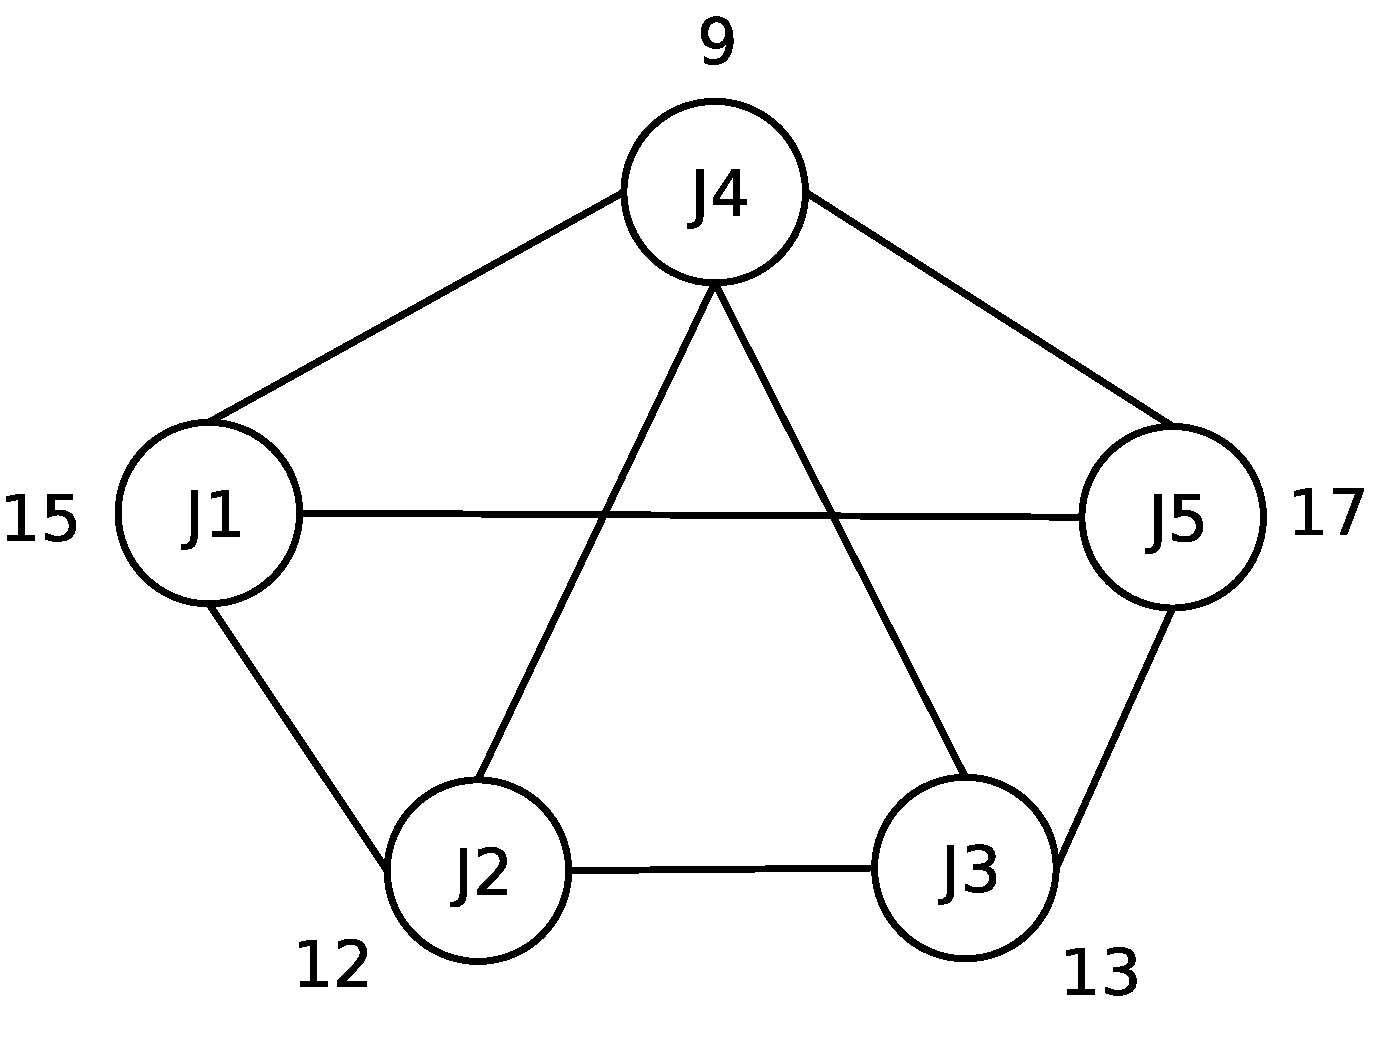
\includegraphics[scale=0.3]{./fig/graph.pdf}
  \caption{Grafo de tarefas da Tabela \ref{tabela:tarefamaquina}.}
  \label{fig:graph}
\end{figure}

A cada iteração as formigas irão percorer o grafo da Figura \ref{fig:graph}, formando uma sequência de tarefas (nós), cujo o 
\textit{makespan} seja o menor possível. Durante o percurso, elas depositam feromônio nas trilhas (arcos) que percorrem 
indicando caminhos para boas soluções. O feromônio e o valor do nó influenciam na escolha da rota seguida por
cada formiga.



% implementacao
\section{Implementação.}
As três classes principais da implementação da Meta-heurística de Colônia de Formigas são apresentadas
na Figura \ref{fig:modelo_aep}.

\begin{figure}[ht]
  \centering
  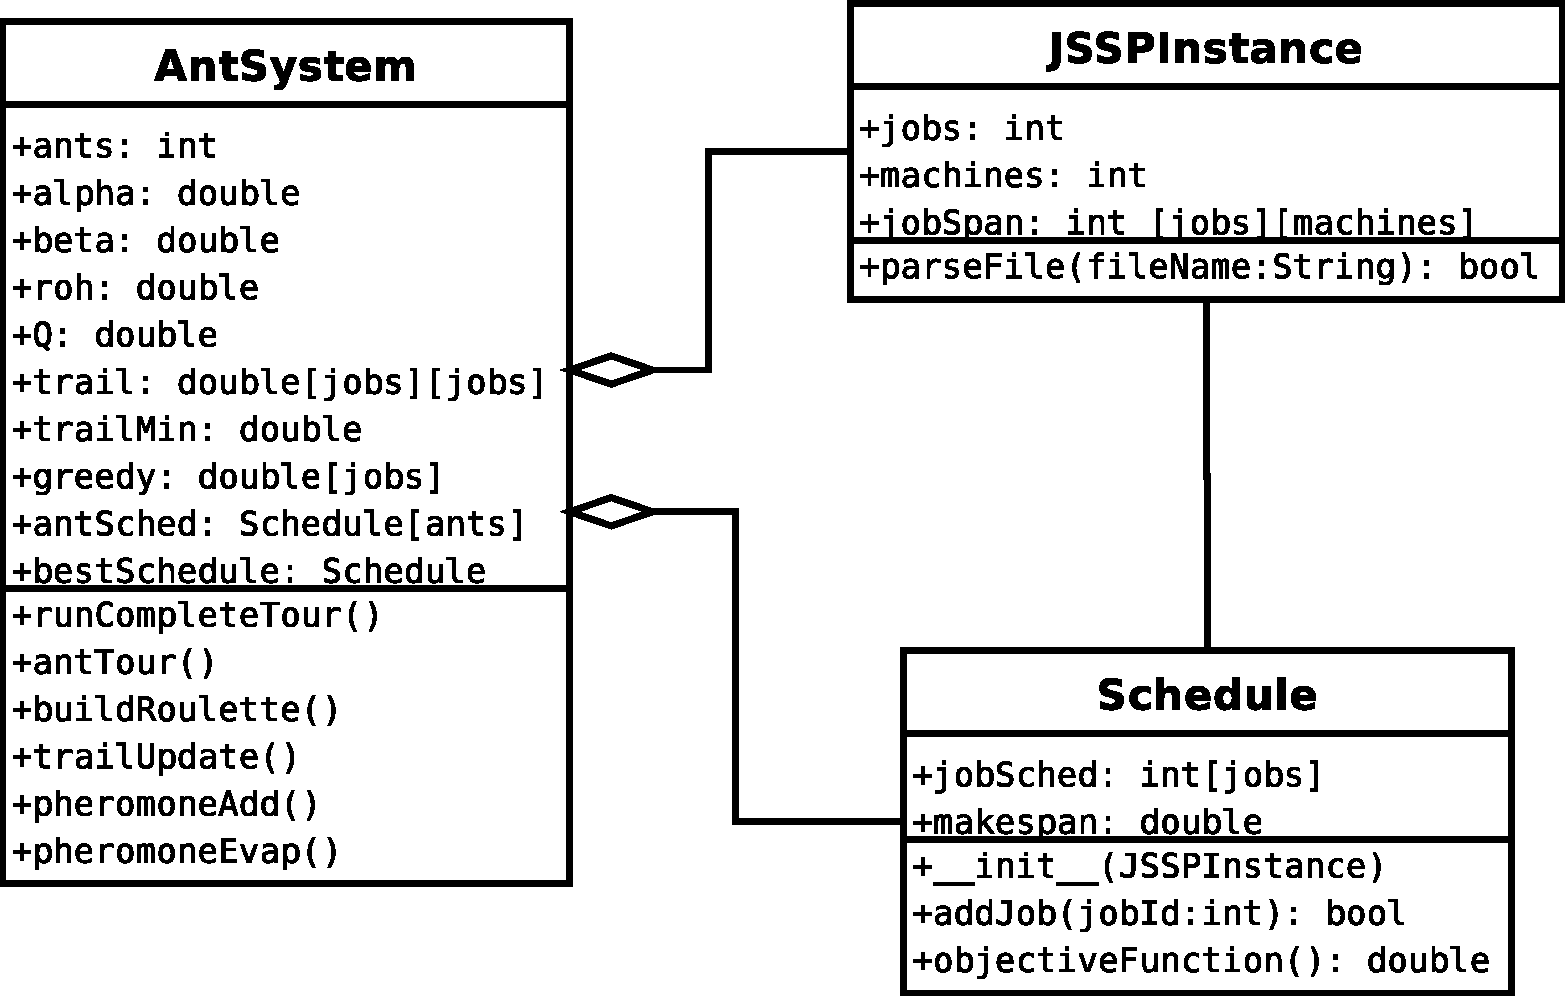
\includegraphics[scale=0.4]{./fig/modelo_aep.pdf}
  \caption{Principais classes da implementação.}
  \label{fig:modelo_aep}
\end{figure}

O núcleo da implementação está na classe AntSystem, que contém todo o código associado a Meta-heurística
de Colônia de Formigas.
A classe JSSPInstance é a responável por ler o arquivo com a instância do problema. A classe Schedule
contém uma sequência de tarefas que formam uma solução válida, ela também é responsável por calcular
o \textit{makespan} associado a sua solução.


\subsection{Customizações.}
Algumas mudanças foram introduzidas nesta implementação, a fim de melhorar seu desempenho,
tornando-a ligeiramente diferente da proposta original \cite{colorni1994ant}.

Uma das mudanças foi na função que adiciona feromônio às rotas percorridas pelas formigas. A implementação
original, também conhecida como elitista, adiciona feromônio a todos os arcos percorridos pelas formigas em 
uma iteração de forma proporcional a qualidade da solução obtida. Contudo, verificou-se que um número elevado
de iterações é necessário para que o nível de feromônio em uma rota se destaque dos demais. Para acelerar este 
processo, adicionamos feromônio apenas nos arcos que compõem a melhor solução da iteração. Ou seja, se existirem
dez formigas decobrindo dez rotas por iteração, apenas uma delas, a melhor, receberá feromônio.

Um ponto sem consenso em \cite{colorni1994ant} e \cite{Zwaan99antcolony} é o valor de inicialização de feromônio.
Adotou-se a estratégia de inicializá-los com o inverso do somatório dos tempos totais de cada tarefa, ver \eqref{eq:trail_min}.
Desta forma, inicializa-se cada arco o valor de feromônio relativo a pior solução possível, solução onde as tarefas são executadas
sequencialmente sem paralelismo.

\begin{equation} \label{eq:trail_min}
Feromonio_{ini,min} = \frac{1}{\sum_{j=1}^{jobs}\sum_{m=1}^{maqs}t_{jm}}
\end{equation}

A proposta original \cite{colorni1994ant} não utiliza um valor mínimo de feromônio em um arco. Assim, com o avançar das 
iterações o nível de feromônio em um arco pode chegar muito próximo de zero, praticamente anulando a probabilidade do arco 
ser selecionado. Utiliza-se o valor em \eqref{eq:trail_min} como valor mínimo para manter a um probabilidade baixa, mas não
nula, do arco ser selecionado.

Em \cite{colorni1994ant}, no início de cada iteração as formigas são colocadas em um job(nó) artificial e a partir daí elas 
selecionam qual job irá ocupar a primeira posição de seu \textit{schedule}. Utilizou-se uma estratégia diferente a fim de 
ampliar e intensificar o espaço de busca. Em 70\% das vezes, a posição inicial é definida de forma randômica, no restante 
a formiga inicia na primeira posição da melhor solução. 



% resultados
\section{Resultados}

As instâncias do problema do FlowShop utilizadas com a metaheurística ACO foram
as seguintes


\begin{figure}[htp]
  \begin{center}
    \subfigure[abz5]{\label{fig:edge-a}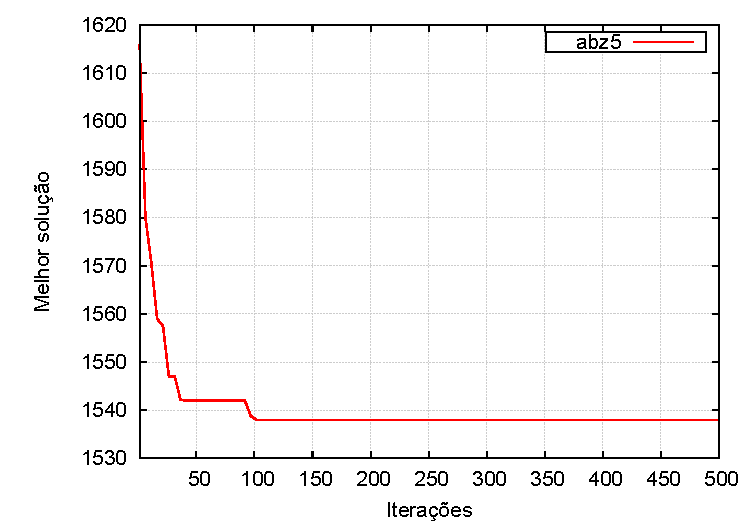
\includegraphics[scale=0.60]{fig/abz5.pdf}}
    \subfigure[car5]{\label{fig:edge-b}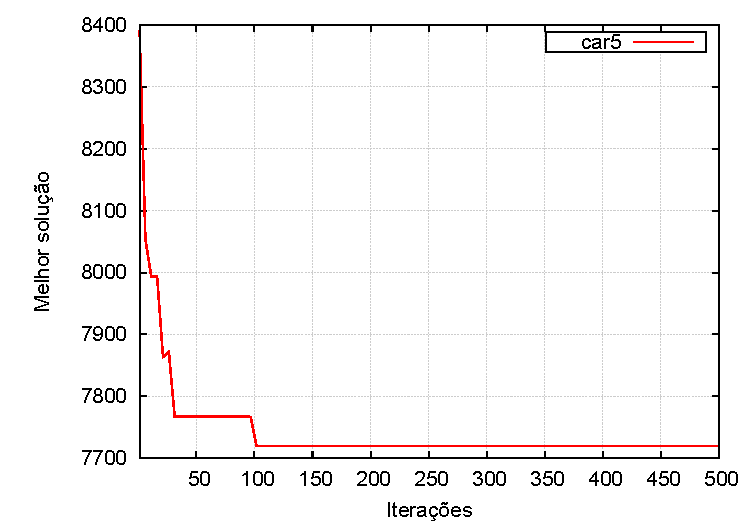
\includegraphics[scale=0.60]{fig/car5.pdf}}
    \\
  \end{center}
  \caption{Convergência do algoritmo Ant-System para as instâncias abz5 e car5}
  \label{fig:edge}
\end{figure}

	\begin{table}
	\centering
	\begin{tabular}{c|c|c|c||c||c|c|c||c}
	\hline\hline
	\multicolumn{4}{c||}{Instâncias Comparativas} & Solução 
	& \multicolumn{3}{|c||}{Solução Obtida} & Aproximação\\
	\hline
	Nº &  Referência & m & n & ``Ótima'' & Inicial & tempo (s) & Melhor & Gap\\
	\hline\hline
	1 & abz5 & 10 & 10 & 1544 & 1592 & 19.7 & 1538 & 0.99611399\\
	2 & car5 & 10 & 6 & 7720 & 8279 & 16.8 & 7720 & 1.0\\
	\hline\hline
	\multicolumn{8}{r||}{Média das aproximações com resultados conhecidos
	$\rightarrowtail$} & 0.998056995	\\
	\hline\hline
	Nº &  Referência & m & n & Inicial & Máxima & Média & Melhor & tempo (s)\\
	\hline\hline
	3 & hel11 & 100 & 10 & 569 & 555 & 552 & 549 & 5636.7 \\
	4 & rec07 & 20 & 10 & 1802 & 1670 & 1635 & 1582 & 51.76 \\
	5 & rec13 & 20 & 15 & 2268 & 2096 & 2052 & 1971 & 57.23 \\
	6 & rec37 & 75 & 20 & 5842 & 5786 & 5753 & 5713 & 2634.3 \\	
	7 & rec41 & 75 & 20 & 6037 & 5892 & 5835 & 5784 & 2656.9 \\
	\hline\hline
	\multicolumn{9}{c}{Instâncias Opcionais} \\
	\hline\hline
	Nº &  Referência & m & n & Inicial & Máxima & Média & Melhor & tempo (s)\\
	\hline\hline
	1 & car1 & 11 & 5 & 7835 & 7038 & 7038 & 7038 & 20.8 \\
	2 & car2 & 13 & 4 & 8148 & 7376 & 7292 & 7166 & 30.4 \\
	3 & car3 & 12 & 5 & 7731 & 7543 & 7425 & 7312 & 26.1 \\
	4 & car4 & 14 & 4 & 8841 & 8423 & 8085 & 8003 & 37.7 \\
	5 & car6 & 8 & 9 & 9588 & 8754 & 8608 & 8505 & 11.3 \\
	6 & car7 & 7 & 7 & 7181 & 6643 & 6621 & 6590 & 7.8 \\
	7 & car8 & 8 & 8 & 9102 & 8564 & 8447 & 8366 & 10.8 \\
	8 & rec01 & 20 & 5 & 1472 & 1360 & 1338 & 1322 & 95.3 \\
	9 & rec03 & 20 & 5 & 1281 & 1188 & 1162 & 1133 & 95.4 \\
	10 & rec05 & 20 & 5 & 1366 & 1284 & 1276 & 1269 & 95.1 \\
	\hline\hline
	\end{tabular}
	\end{table}


% conclusao
\input{conclusao}

\bibliographystyle{plain}	% (uses file "plain.bst")
\bibliography{references}		% expects file "myrefs.bib"


\end{document}
